% GDZ PPN236018647,native497;HKUST498;original diary3v.
% Complete entries corresponding to printed51-53,55,57-58;54/56 excluded.
\clearpage\SourceLeaf{497}\NoSourceHead
\begingroup\fontsize{10}{15}\selectfont\itshape
\newcommand{\DiaryStrike}[1]{\tikz[baseline=(t.base)]{\node[inner sep=0pt,outer sep=0pt] (t) {\strut #1};\draw[line width=.55pt] ([yshift=.15ex]t.west)--([yshift=.15ex]t.east);}}
\noindent Curvam \shortstack[b]{lemniscatam\\\DiaryStrike{elasticam}} a
\(\displaystyle\int\frac{dx}{\surd(1-x^4}\Big)\) pendentem\\
\hspace*{2em}perscrutari cöpi\hfill Jan. 8

\medskip
\noindent Criterii Euleriani rationem sponte detexi\hfill Jan. 10.

\medskip
\noindent Integrale complet. \(\displaystyle\int\frac{dx}{{}^n\!\surd(1-x^n)}\) ad circ. quadr. reducere\\
\hspace*{2em}commentus sum.\hfill Jan. 12.

\medskip
\noindent\underline{Supplementum eximium ad polygonorum descriptio-}\\
\hspace*{2em}\underline{nem inveni. sc. si \(a,b,c,d\) sint factores primi}\\
\hspace*{2em}\underline{numeri primi \raisebox{1ex}{\(p\)} unitate truncati tunc ad polygona \(p\) laterum}\\
\hspace*{2em}\underline{nihil aliud requiri quam ut \(\underline{\underline{1^0}}\) arcus indefinitus in \(a,b,c\)}\\
\hspace*{2em}\underline{\(d\).. partes secetur \(2^0\) ut polygona \(a,b,c,d\).. laterum}\\
\hspace*{2em}\underline{describantur.}\hfill Gotting. Januar. 19

\medskip
\noindent\underline{Forma \(aa+bb+cc\) quod ad divisores}\\
\hspace*{2em}\underline{\(-bc-ac-ab\)}\\
\hspace*{2em}\underline{attinet convenit cum hac \(aa+3bb\)}\hfill Febr. 6

\medskip
\noindent Amplificatio prop. penult. p. 1. scilicet
\[
1-a+a^3-a^6+a^{10}\ldotp\,\ldotp\,\ldotp\,\ldotp\ =\qquad\text{Febr. 16}
\]
\begin{center}
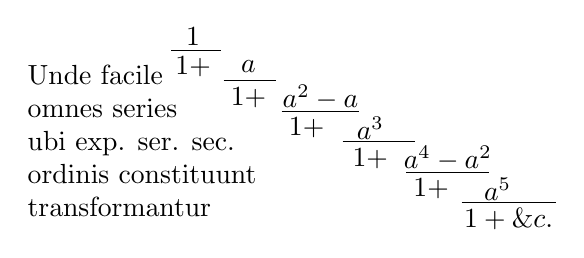
\begin{tikzpicture}[x=1em,y=1em]
\node[anchor=north west,align=left,inner sep=0] at (-6,-1) {Unde facile\\omnes series\\ubi exp. ser. sec.\\ordinis constituunt\\transformantur};
\node[inner sep=0] at (0,0) {\(1\)};
\draw (-.8,-.5)--(1,-.5);
\node[inner sep=0] at (0,-1.1) {\(1+\)};
\node[inner sep=0] at (2,-1.1) {\(a\)};
\draw (1.1,-1.6)--(3,-1.6);
\node[inner sep=0] at (2,-2.2) {\(1+\)};
\node[inner sep=0] at (4.6,-2.2) {\(a^2-a\)};
\draw (3.2,-2.7)--(6,-2.7);
\node[inner sep=0] at (4.1,-3.3) {\(1+\)};
\node[inner sep=0] at (6.4,-3.3) {\(a^3\)};
\draw (5.4,-3.8)--(8,-3.8);
\node[inner sep=0] at (6.4,-4.4) {\(1+\)};
\node[inner sep=0] at (9.2,-4.4) {\(a^4-a^2\)};
\draw (7.7,-4.9)--(10.7,-4.9);
\node[inner sep=0] at (8.6,-5.5) {\(1+\)};
\node[inner sep=0] at (11,-5.5) {\(a^5\)};
\draw (9.7,-6)--(13.1,-6);
\node[inner sep=0] at (11.4,-6.6) {\(1+\text{\&c.}\)};
\end{tikzpicture}
\end{center}
\endgroup
